% !TEX root = ../thesis.tex
\graphicspath{{\aiaadir /figures_flatplate/}}% Set graphics path location

\subsection{Subsonic laminar flat-plate}

Computations of the flow over a subsonic flat-plate have been performed and validated against the Blasius' solution for laminar boundary layer. The flow conditions are \gls{ma} $0.5$, 0$\degr$ angle of attack and \gls{re} $1\cdot10^6$ based on the plate length. The governing equations are the 2D \gls{ns} equations with constant ratio of specific heats of $1.4$, Prandtl number of $0.72$ and constant dynamic viscosity of $1.827\cdot 10^{-5} Pa \cdot s$.

\begin{center} 
    \begin{tabular}{l*{7}{c}r}
    Mesh & First cell height & \specialcell{\# of cells in \vspace{0.2cm}\\boundary layer} & $p_3$ & $p_4$ & $p_5$ & $p_6$ \\ \hline
    Mesh a0 (140 = 14x10) & 0.00075 & 2 & $\times$ & $\times$ & $\times$ & \Checkmark \\ \hline
    Mesh a1 (560 = 28x20) & 0.000375 & 4 &  $\times$ & $\times$ & \Checkmark & \Checkmark \\ \hline
    Mesh a2 (2240 = 56x40) & 0.0001875 & 8 & $\times$ & \Checkmark & \Checkmark & \Checkmark \\ \hline
    Mesh a3 (8960 = 112x80) & 0.0000935 & 16 & \Checkmark & \Checkmark & \Checkmark & \Checkmark \\
    \hline
    \end{tabular} 
      \captionof{table}{\gls{hf} convergence using different grids and polynomial order. $\times$ / \Checkmark indicates not converged/converged resp.} \label{tab:convergence} 
\end{center}

The objective of this study is to determine the minimum number of elements and the order of polynomial required to converge the flat-plate simulation using \gls{hf}. Four different numerical grids have been used in this study (2, 4, 8, 16 elements inside the boundary layer) and four polynomial orders ($p_3$--$p_6$). The results, summarized in Table \ref{tab:convergence}, show that a minimum number of elements is needed in the boundary layer depending on the polynomial order to obtain satisfactory convergence (free from inter-element jumps).

\begin{figure}
\begin{center}
\begin{minipage}[t]{0.48\columnwidth}
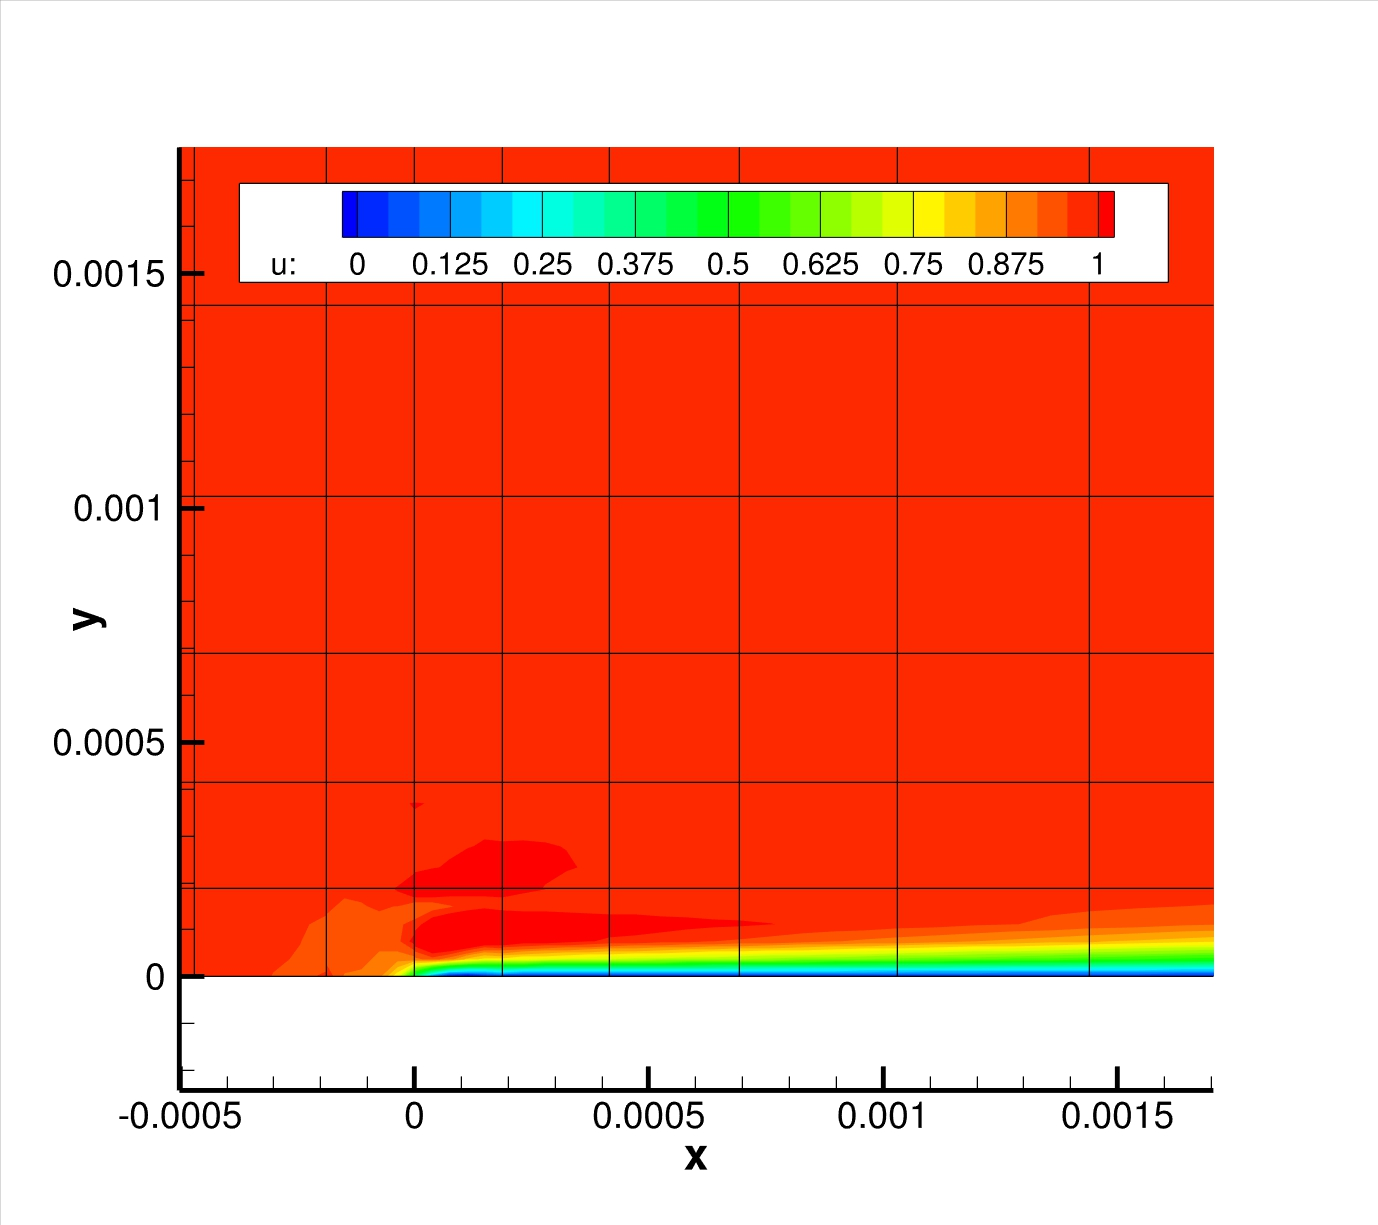
\includegraphics[width = \textwidth,clip=]{LeadingEdge.jpg}
\caption{Detail of the flat-plate leading edge (x=0.0, mesh a2).}
\label{fig:LeagingEdge}
\end{minipage}
\hfill
\begin{minipage}[t]{0.48\columnwidth}
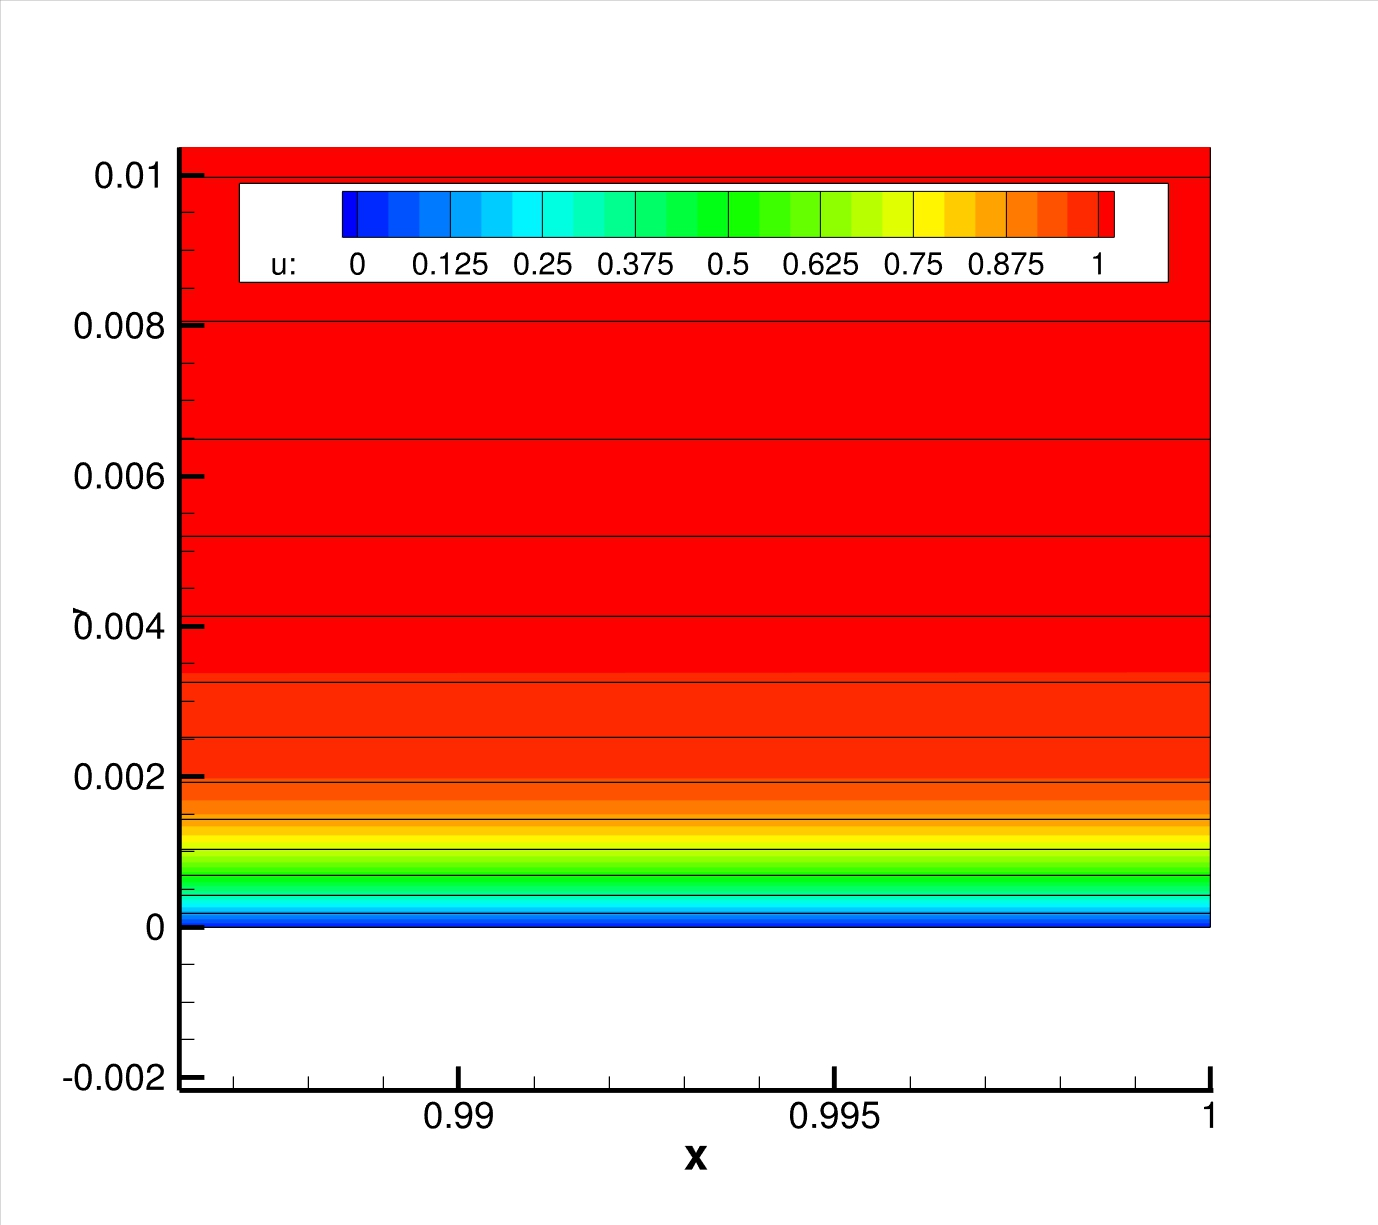
\includegraphics[width = \textwidth,clip=] {EndPlate.jpg}
\caption{Flow solution at the end of the flat-plate (x=1.0, mesh a2).}
\label{fig:TrailingEdge}
\end{minipage}
\end{center}
\end{figure}

The results are compared with the Blasius' solution for laminar boundary layer with satisfactory results, and some details of the solutions are presented in Fig. \ref{fig:LeagingEdge} (leading edge), and Fig. \ref{fig:TrailingEdge} (end of the flat-plate). It is important to note that in this particular case (mesh a2) the flat-plate boundary layer is captured using 8 elements, while in a second order solver it would be necessary of the order of ~30 elements inside the boundary layer.

\begin{figure}
\begin{center}
\begin{minipage}[t]{0.48\columnwidth}
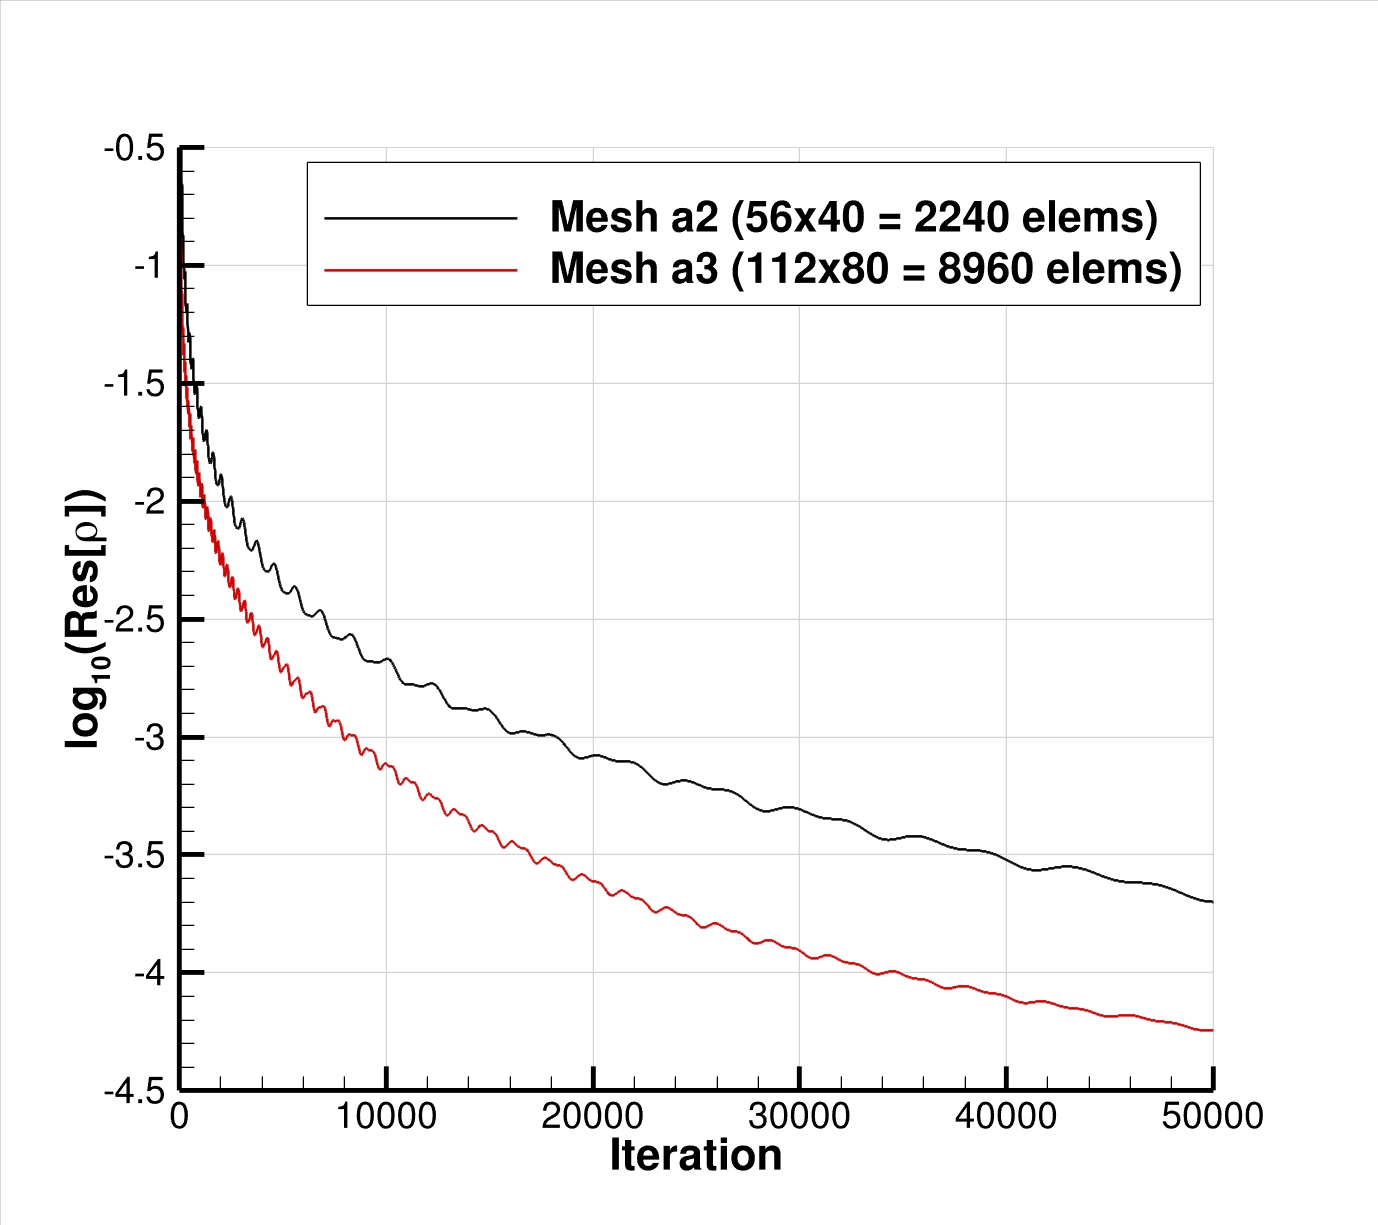
\includegraphics[width = \textwidth]{CompMesh.jpg}
\caption{Convergence comparison (3$^{rd}$ order, finest grids).}
\label{fig:ComparisonOrder}
\end{minipage}
\hfill
\begin{minipage}[t]{0.48\columnwidth}
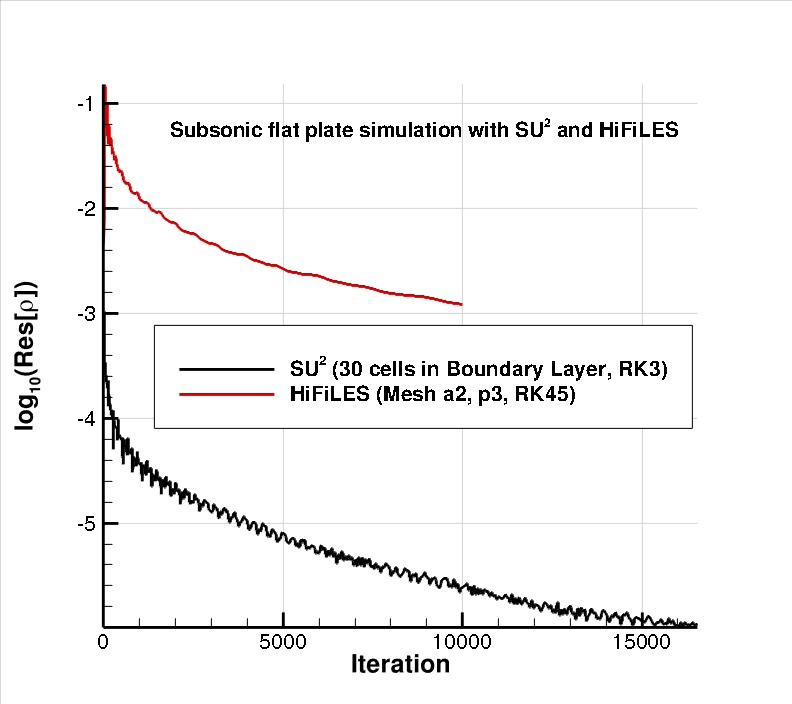
\includegraphics[width = \textwidth] {CompSu2.jpg}
\caption{Comparison of \gls{hf} with SU2 using a similar time integration scheme.}
\label{fig:Comparison_SecondOrder}
\end{minipage}
\end{center}
\end{figure}

To finalize, it is critical to note that the absence of a local time stepping technique in \gls{hf} increases the required number of iterations to obtain a converged solution. However, we have noticed an improvement of the rate of convergence as we refine the grid (see Fig. \ref{fig:ComparisonOrder}). The obtained convergence rate is comparable to a second order numerical code (e.g. SU2~\cite{palacios2013stanford,palacios14}) running using a similar numerical time integration (see Fig.~\ref{fig:Comparison_SecondOrder}).
